\section{Existing system}

The Department of Astronomy and Astrophysics
(DAA), Faculty of Mathematics, Physics and Informatics of Comenius University in Bratislava, Slovakia uses a 70 cm Newtonian telescope \ref{fig:telescope} for observation and developed system for tracking space debris and other objects.

Object catalogization consists of these steps \cite{krajvcovivc2019selected}:
\begin{enumerate}
    \item Star field identification\\
    Star field is identification with Astrometry.NET scripts
    \item Image reduction\\ 
    Removing multiplicative errors from the image caused by imperfect circumstances. These errors are removed by subtracting \textit{bias} frame (taken with closed shutter).
    \item Background estimation and subtraction\\
    Sigma clipping is used to estimate and subtract background from the image
    \item Objects search and centroiding (segmentation)\\
    Object are detected in the image and their position and other attributes are saved in text file.
    \item Astrometric reduction\\
    Position of the object from previous step is translated to the equatorial coordinates.
    \item Masking\\
    Masking is used to remove duplicate and stationary objects
    \item Tracklet building\\
    Finding trajectory of moving objects
    \item Object identification\\
    Identification of the object in the catalogue

\end{enumerate}

\begin{figure}[h!]
    \centering
    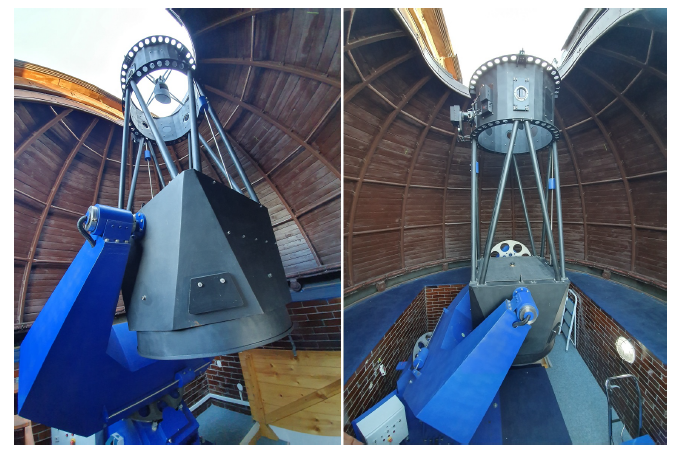
\includegraphics[width=60mm]{chapters/images/telescope.PNG}
    \caption{Telescope}
    \label{fig:telescope}
\end{figure}


\subsection{Tracklet building}

I am focused on tracklet building in my thesis. Tracklet is a data structure containing consecutive observations of a frame object in time. We can refer to tracklet as trajectory of the object. 

\begin{figure}[h!]
    \centering
    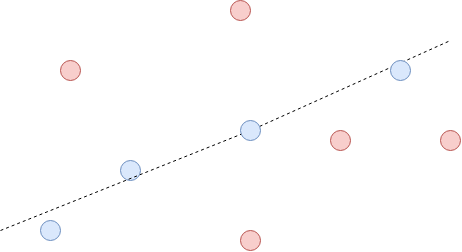
\includegraphics[width=100mm]{chapters/images/trajectory_img.png}
    \caption{Trajectory and tracklet of object}
    \label{fig:TB_trajectory}
\end{figure}

Blue object in the figure \ref{fig:TB_trajectory} are representing tracklet and red object are points which were not chosen to tracklet. We can then approximate this positions by imaginary line which represents trajectory of object in time and space.

We can approximate object trajectory by line as we are observing only small part of sky where true trajectories of object in Earth orbit are very close to simple line. 

In this system, Simple linear regression (SLR)  is used to find sequence of object on a line \cite{krajvcovivc2019selected}. Tracklet building is then realized in following steps:
\begin{enumerate}
    \item Creating Cartesian product of objects from first and second frame
    \item Computing angular velocity and position angle of two point for every couple
    \item For each k-tuple we check if exists object in the next frame with position close to computed next position from previous step. This object is added to tracklet.
    \item Line parameters for k-tuples are updated with SLR
    \item Continue iteratively on step 3
\end{enumerate}

After processing object from all frames tracklets are saved to text file. 


\subsection{Equatorial coordinate system}

Position of object after \textit{Astrometric reduction} is given in Equatorial coordinates. Equatorial coordinates represents position  of object on celestial sphere \cite{thompson2006coordinate} . 

\begin{figure}[!h]
    \centering
    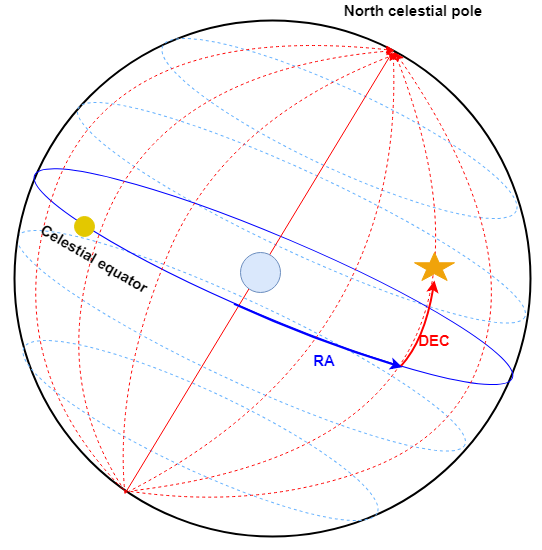
\includegraphics[width=100mm]{chapters/images/equatorial_coordinates.png}
    \caption{Equatorial coordinates of object}
    \label{fig:Equatorial_coordinates}
\end{figure}

Position consists of two coordinates. 
\begin{itemize}
    \item \textbf{Declination} - measures the angular distance from celestial equator. Declination has values from $-90°$ up to $+90°$. $-90°$ value represents South pole and $+90°$ the North pole.
    \item \textbf{Right ascension} - measures angular distance from Greenwich meridian along celestial equator. Right ascension is usually measured in sidereal hours from $0$ hour $0 min$ $0$ sec to $24$ hour. For easier manipulation can be rewritten as angle.
\end{itemize}

Position of object in equatorial or heliographic coordinates are computed in astrometric reduction with use of information from FITs header (FITs images are made by telescope).

Although equatorial coordinates do not represent position on 2-D plane, as our filed of observation is very small we can assume that Equatorial coordinates behaves such as Euclidean coordinates. 
